\section{Creating C++ Applications}

Not everyone wants a full blown GIS desktop application. Sometimes you want
to just have a widget inside your application that displays a map while the
main goal of the application lies elsewhere. Perhaps a database frontend with
a map display? This Section provides two simple code examples by Tim Sutton. 
They are available in the qgis subversion repository together with more
interesting tutorials. Check out the whole repository from: 
\filename{https://svn.osgeo.org/qgis/trunk/code\_examples/}

\subsection{Creating a simple mapping widget}\label{subsec:simple_widget}

With this first tutorial we take a little walk through creating a simple mapping
widget. It won't do anything much - just load a shape file and display it in
a random colour. 
But it should give you an idea of the potential for using QGIS as an embedded
mapping component. Before we carry on, many thanks to Francis Bolduc who wrote
the beginnings of this demo. He kindly agreed to make his work generally
available.

We start with typical adding the neccessary includes for our app:

\begin{verbatim}
//
// QGIS Includes
//
#include <qgsapplication.h>
#include <qgsproviderregistry.h>
#include <qgssinglesymbolrenderer.h>
#include <qgsmaplayerregistry.h>
#include <qgsvectorlayer.h>
#include <qgsmapcanvas.h>
//
// Qt Includes
//
#include <QString>
#include <QApplication>
#include <QWidget>
\end{verbatim}

We use QgsApplication instead of Qt's QApplication, and get some added
benifits of various static methods that can be used to locate library paths
and so on.

The provider registry is a singleton that keeps track of vector data provider
plugins. It does all the work for you of loading the plugins and so on. The
single symbol renderer is the most basic symbology class. It renders points,
lines or polygons in a single colour which is chosen at random by default
(though you can set it yourself). Every vector layer must have a symbology
associated with it.

The map layer registry keeps track of all the layers you are using. The
vector layer class inherits from maplayer and extends it to include
specialist functionality for vector data.

Finally the mapcanvas is really the nub of the matter. Its the drawable
widget that our map will be drawn onto.

Now we can move on to initialising our application....

\begin{verbatim}
int main(int argc, char ** argv)
{
  // Start the Application
  QgsApplication app(argc, argv, true);

  QString myPluginsDir        = "/home/timlinux/apps/lib/qgis";
  QString myLayerPath         = "/home/timlinux/gisdata/brazil/BR_Cidades/";
  QString myLayerBaseName     = "Brasil_Cap";
  QString myProviderName      = "ogr";

\end{verbatim}

So now we have a qgsapplication and we have defined some variables. Since I
tested this on the Ubuntu 8.10, I just specified the location of the vector
provider plugins as being inside the my development install directory. It
would probaby make more sense in general to keep the QGIS libs in one of the
standard library search paths on your system (e.g. /usr/lib) but this way
will do for now.

The next two variables defined here just point to the shapefile I am going to
be using (and you should substitute your own data here).

The provider name is important - it tells qgis which data provider to use to
load the file. Typically you will use 'ogr' or 'postgres'.

Now we can go on to actually create our layer object.

\begin{verbatim}
  // Instantiate Provider Registry
  QgsProviderRegistry::instance(myPluginsDir);
\end{verbatim}

First we get the provider registry initialised. Its a singleton class so we
use the static instance call and pass it the provider lib search path. As it
initialises it will scan this path for provider libs.

Now we go on to create a layer...

\begin{verbatim}
  QgsVectorLayer * mypLayer =
      new QgsVectorLayer(myLayerPath, myLayerBaseName, myProviderName);
  QgsSingleSymbolRenderer *mypRenderer = new
QgsSingleSymbolRenderer(mypLayer->geometryType());
  QList <QgsMapCanvasLayer> myLayerSet;

  mypLayer->setRenderer(mypRenderer);
  if (mypLayer->isValid())
  {
    qDebug("Layer is valid");
  }
  else
  {
    qDebug("Layer is NOT valid");
  }

  // Add the Vector Layer to the Layer Registry
  QgsMapLayerRegistry::instance()->addMapLayer(mypLayer, TRUE);
  // Add the Layer to the Layer Set
  myLayerSet.append(QgsMapCanvasLayer(mypLayer, TRUE));

\end{verbatim}

The code is fairly self explanatory here. We create a layer using the
variables
we defined earlier. Then we assign the layer a renderer. When we create a
renderer, we need to specify the geometry type, which do do by asking the
vector layer for its geometry type. Next we add the layer to a layerset
(which
is used by the QgsMapCanvas to keep track of which layers to render and in
what
order) and to the maplayer registry. Finally we make sure the layer will be
visible.

Now we create a map canvas on to which we can draw the layer.

\begin{verbatim}
  // Create the Map Canvas
  QgsMapCanvas * mypMapCanvas = new QgsMapCanvas(0, 0);
  mypMapCanvas->setExtent(mypLayer->extent());
  mypMapCanvas->enableAntiAliasing(true);
  mypMapCanvas->setCanvasColor(QColor(255, 255, 255));
  mypMapCanvas->freeze(false);
  // Set the Map Canvas Layer Set
  mypMapCanvas->setLayerSet(myLayerSet);
  mypMapCanvas->setVisible(true);
  mypMapCanvas->refresh();

\end{verbatim}

Once again there is nothing particularly tricky here. We create the canvas
and then we set its extents to those of our layer. Next we tweak the canvas a bit
to draw antialiased vectors. Next we set the background colour, unfreeze the
canvas, make it visible and then refresh it.

\begin{verbatim}
  // Start the Application Event Loop
  return app.exec();
}

\end{verbatim}

In the last step we simply start the Qt event loop and we are all done. You
can check out, compile and run this example using cmake like this:

\begin{verbatim}
svn co
https://svn.osgeo.org/qgis/trunk/code_examples/1_hello_world_qgis_style
cd 1_hello_world_qgis_style
mkdir build
#optionally specify where your QGIS is installed (should work on all
platforms)
#if your QGIS is installed to /usr or /usr/local you can leave this next step
out
export LIB_DIR=/home/timlinux/apps
cmake ..
make
./timtut1
\end{verbatim}

When we compile and run it here is what the running app looks like:

\begin{figure}[ht]
   \begin{center}
   \caption{Simple C++ Application \osxcaption}\label{fig:cpp1_application}\smallskip
   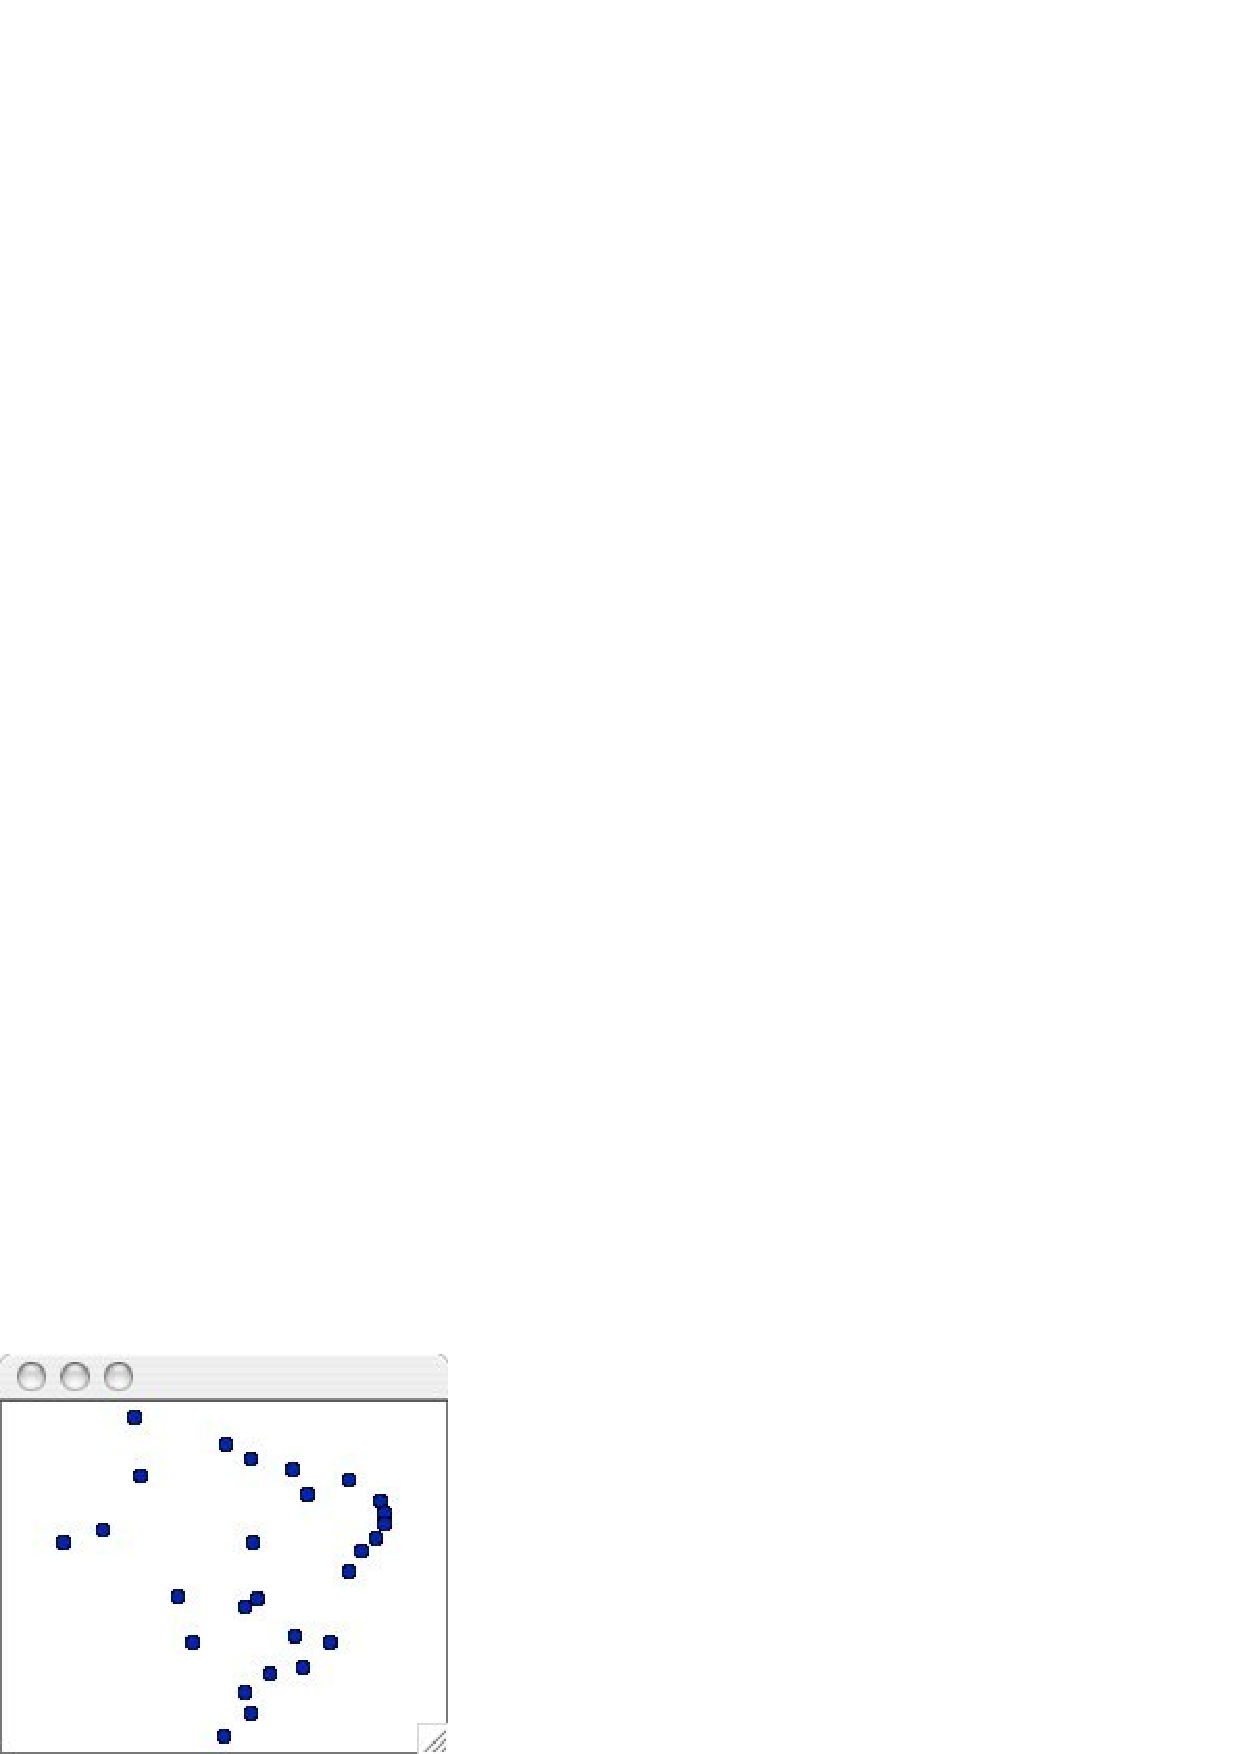
\includegraphics[clip=true]{cpp1_application}
\end{center}
\end{figure}

\subsection{Working with QgsMapCanvas}

In Section~\ref{subsec:simple_widget} we showed you the usage of the
QgsMapCanvas api to create a simple application that loads a shapefile and
displays the points in it. But what good is a map that you can't interact
with? 

In this second tutorial I will extend the last tutorial by making it a
QMainWindow application with a menu, toolbar and canvas area. We show you how
to use QgsMapTool - the base class for all tools that need to interact with
the map canvas.
The purpose is to provide a demonstrator project, so I wont promise to write the most
elegant or robust C++ code. The project will provide 4 toolbar icons for

\begin{itemize}
 \item loading a map layer (layer name is hard coded in the application
 \item zooming in
 \item zooming out
 \item panning
\end{itemize}

In the working directory for the tutorial code you will find a number of files
including c++ sources, icons and a simple data file under data. There is also
the .ui file for the main window.

\textbf{Note:} You will need to edit the .pro file in the above svn directory to
match your system.

Since much of the code is the same as the previous tutorial, I will focus on
the MapTool specifics - the rest of the implementation details can be
investigated by checking out the project form SVN. A QgsMapTool is a class that
interacts with the MapCanvas using the mouse pointer. QGIS has a number of
QgsMapTools implemented, and you can subclass QgsMapTool to create your own. In
mainwindow.cpp you will see I include the headers for the QgsMapTools near the
start of the file:

\begin{verbatim}
     //
     // QGIS Map tools
     //
     #include "qgsmaptoolpan.h"
     #include "qgsmaptoolzoom.h"
     //
     // These are the other headers for available map tools 
     // (not used in this example)
     //
     //#include "qgsmaptoolcapture.h"
     //#include "qgsmaptoolidentify.h"
     //#include "qgsmaptoolselect.h"
     //#include "qgsmaptoolvertexedit.h"
     //#include "qgsmeasure.h"
\end{verbatim}

As you can see, I am only using two types of MapTool subclasses for this
tutorial, but there are more available in the QGIS library. Hooking up our
MapTools to the canvas is very easy using the normal Qt4 signal/slot mechanism:

\begin{verbatim}
     //create the action behaviours
     connect(mActionPan, SIGNAL(triggered()), this, SLOT(panMode()));
     connect(mActionZoomIn, SIGNAL(triggered()), this, SLOT(zoomInMode()));
     connect(mActionZoomOut, SIGNAL(triggered()), this, SLOT(zoomOutMode()));
     connect(mActionAddLayer, SIGNAL(triggered()), this, SLOT(addLayer()));
\end{verbatim}

Next we make a small toolbar to hold our toolbuttons. Note that the mpAction*
actions were created in designer.

\begin{verbatim}
     //create a little toolbar
     mpMapToolBar = addToolBar(tr("File"));
     mpMapToolBar->addAction(mpActionAddLayer);
     mpMapToolBar->addAction(mpActionZoomIn);
     mpMapToolBar->addAction(mpActionZoomOut);
     mpMapToolBar->addAction(mpActionPan);
\end{verbatim}

Thats really pretty straightforward Qt stuff too. Now we create our three map
tools:

\begin{verbatim}
     //create the maptools
     mpPanTool = new QgsMapToolPan(mpMapCanvas);
     mpPanTool->setAction(mpActionPan);
     mpZoomInTool = new QgsMapToolZoom(mpMapCanvas, FALSE); // false = in
     mpZoomInTool->setAction(mpActionZoomIn);
     mpZoomOutTool = new QgsMapToolZoom(mpMapCanvas, TRUE ); //true = out
     mpZoomOutTool->setAction(mpActionZoomOut);
\end{verbatim}

Again nothing here is very complicated - we are creating tool instances, each
of which is associated with the same mapcanvas, and a different QAction. When
the user selects one of the toolbar icons, the active MapTool for the canvas is
set. For example when the pan icon is clicked, we do this:

\begin{verbatim}
    void MainWindow::panMode()
    {
       mpMapCanvas->setMapTool(mpPanTool); 
    }
\end{verbatim}

\begin{figure}[ht]
   \begin{center}
   \caption{QMainWindow application with a menu, toolbar and canvas area
\osxcaption}\label{fig:cpp2_application}\smallskip
   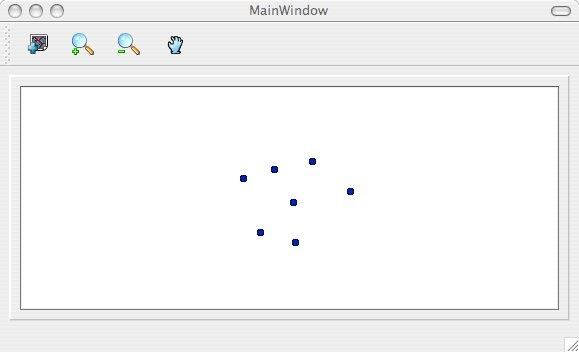
\includegraphics[clip=true, width=\textwidth]{cpp2_application}
\end{center}
\end{figure}

\minisec{Conclusion}

As you can see extending our previous example into something more functional
using MapTools is really easy and only requires a few lines of code for each
MapTool you want to provide.

You can check out and build this tutorial using SVN and CMake using the following steps:

\begin{verbatim}
svn co https://svn.osgeo.org/qgis/trunk/code_examples/2_basic_main_window
cd 2_basic_main_window
mkdir build
#optionally specify where your QGIS is installed (should work on all platforms)
#if your QGIS is installed to /usr or /usr/local you can leave this next step out
export LIB_DIR=/home/timlinux/apps
cmake ..
make
./timtut2
\end{verbatim}


